% This file was created by matlab2tikz.
%
%The latest updates can be retrieved from
%  http://www.mathworks.com/matlabcentral/fileexchange/22022-matlab2tikz-matlab2tikz
%where you can also make suggestions and rate matlab2tikz.
%
\documentclass[tikz]{standalone}
\usepackage[T1]{fontenc}
\usepackage[utf8]{inputenc}
\usepackage{pgfplots}
\usepackage{grffile}
\pgfplotsset{compat=newest}
\usetikzlibrary{plotmarks}
\usetikzlibrary{arrows.meta}
\usepgfplotslibrary{patchplots}
\usepackage{amsmath}

\begin{document}
\definecolor{mycolor1}{rgb}{0.00000,0.44700,0.74100}%
%
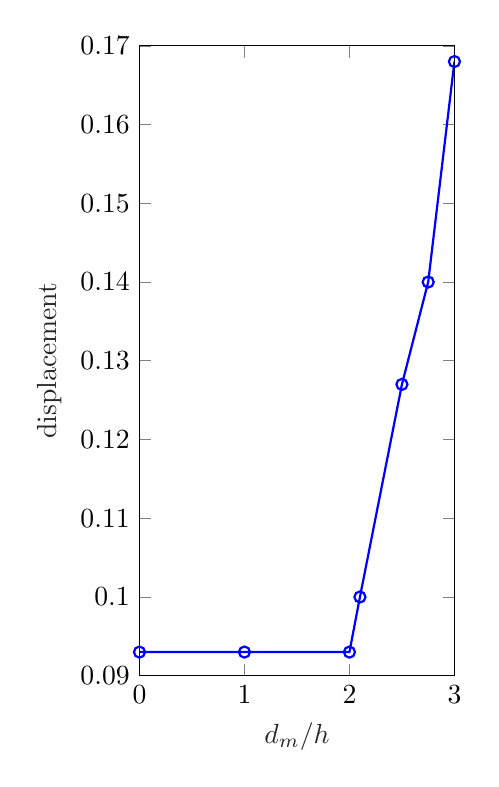
\begin{tikzpicture}

\begin{axis}[%
width=4cm,
height=8cm,
at={(0cm,0cm)},
scale only axis,
xmin=0.000,
xmax=3.000,
xlabel style={font=\color{white!15!black}},
xlabel={$d_m/h$},
ymin=0.090,
ymax=0.170,
yticklabel style={
        /pgf/number format/fixed,
        /pgf/number format/precision=2
},
ylabel style={font=\color{white!15!black}},
ylabel={displacement},
axis background/.style={fill=white}
]
\addplot [blue, style = {thick}, mark=o, mark options={solid, thick}, forget plot]
  table[row sep=crcr]{%
0.000	0.093\\
1.000	0.093\\
2.000	0.093\\
2.100	0.100\\
2.500	0.127\\
2.750	0.140\\
3.000	0.168\\
};
\end{axis}
\end{tikzpicture}%
\end{document}